% !BIB TS-program = biber
\documentclass[pdftex,12pt,a4paper,twoside]{book}

\usepackage[utf8]{inputenc}
\usepackage[ngerman, english]{babel}
%\usepackage{microtype}% verbesserter Randausgleich
\usepackage[heightrounded]{geometry}
\geometry{a4paper, left=2.5cm, right=2.5cm, top=2.5cm, bottom=2.5cm}
\setlength{\parindent}{0cm}
\setlength{\footskip}{1cm} 
\newcommand{\HRule}{\rule{\linewidth}{0.5mm}}
\usepackage[font=footnotesize,labelfont=bf,format=plain]{caption}
\captionsetup{labelsep=space,labelfont=bf}
\usepackage[font=footnotesize]{subcaption}
\usepackage[pdftex]{graphicx}
\usepackage{verbatim}
\usepackage{csvsimple}
\usepackage{pgfplotstable}
\usepackage{hyperref}
\usepackage{cleveref}
\usepackage{fancyhdr}
\usepackage{booktabs}
\usepackage{amsfonts} 
\renewcommand{\cite}{\shortcite}
%\usepackage[sort&compress,comma,super,square]{natbib}
\usepackage[export]{adjustbox}
\usepackage{pdfpages}
\usepackage[
    %backend=biber, 
    natbib=true,
    style=numeric,
    sorting=none
]{biblatex} %Imports biblatex package
\addbibresource{refs.bib} %Import the bibliography file

\newcommand\mycaption[2]{\caption{\textbf{#1}\newline\small#2}}


\newcommand{\beginsupplement}{%
	\setcounter{table}{0}
	\renewcommand{\thetable}{S\arabic{table}}%
	\setcounter{figure}{0}
	\renewcommand{\thefigure}{S\arabic{figure}}%
}

\pgfplotstableset{
	col sep=tab,
	string type,
	every head row/.style={after row=\toprule, before row=\midrule},
	every last row/.style={after row=\bottomrule}
}

\usepackage{titlesec, color}
\usepackage{titlesec}
  
\definecolor{gray75}{gray}{0.75}
\newcommand{\hsp}{\hspace{20pt}}
%\titleformat{\chapter}[hang]{\Huge\bfseries}{\thechapter\vspace{2em}}{0pt}{\Huge\bfseries}
\setcounter{tocdepth}{3}
%\setcounter{secnumdepth}{3}
\begin{document}

\begin{titlepage}

%%LR
\sffamily

\begin{center}

% Oberer Teil der Titelseite:

\includegraphics[left]{logos/ETHlogo.pdf}
\\[5cm]

{\Large Study Program}\\[0.5cm]
{\Large ETH Z{\"u}rich}\\[0.5cm]
{\Large Master Thesis}\\[2.5cm]

% Title
\HRule \\[0.4cm]
{ \huge \bfseries  Thesis Title}\\[0.4cm]

\HRule \\[1.5cm]

{\Large Max Mustermann}\\[2.5cm]

\vfill
\end{center}
\end{titlepage}
\pagestyle{empty}


%%LR comprehensive title
\begin{titlepage}
{\sffamily


\begin{center}
% Oberer Teil der Titelseite:

\includegraphics[left]{logos/ETHlogo.pdf}
\\[5cm]

{\Large Study Program}\\[0.5cm]
{\Large ETH Z{\"u}rich}\\[0.5cm]
{\Large Master Thesis}\\[2.5cm]

% Title

{ \huge \bfseries  Thesis Title}\\[0.4cm]


\vfill
\end{center}

\begin{center}\Large
  \begin{tabular}{ll}
    Author:& Max Mustermann\\
    Supervisor: & Prof. Mustermann, \\
			    & ETH Z{\"u}rich, Department of Computer Science\\
    Advisor:    & Max Mustermann,\\
			    & ETH Z{\"u}rich, Department of Computer Science\\
    Submitted:  &  28.08.2023
  \end{tabular}
\end{center}


}% end title page
\end{titlepage}
\pagestyle{empty}



%%LR comprehensive title
\begin{titlepage}
{\sffamily



}% end title page

\end{titlepage}

\newpage~

%%%%%%%%%%%%%%%%%%%%%%%%%%%%%%%%%
% thesis content starts here
%%%%%%%%%%%%%%%%%%%%%%%%%%%%%%%%%


\newgeometry{a4paper, left=3cm, right=3cm, top=3.5cm, bottom=3.5cm}
\pagestyle{headings}
\pagenumbering{roman}
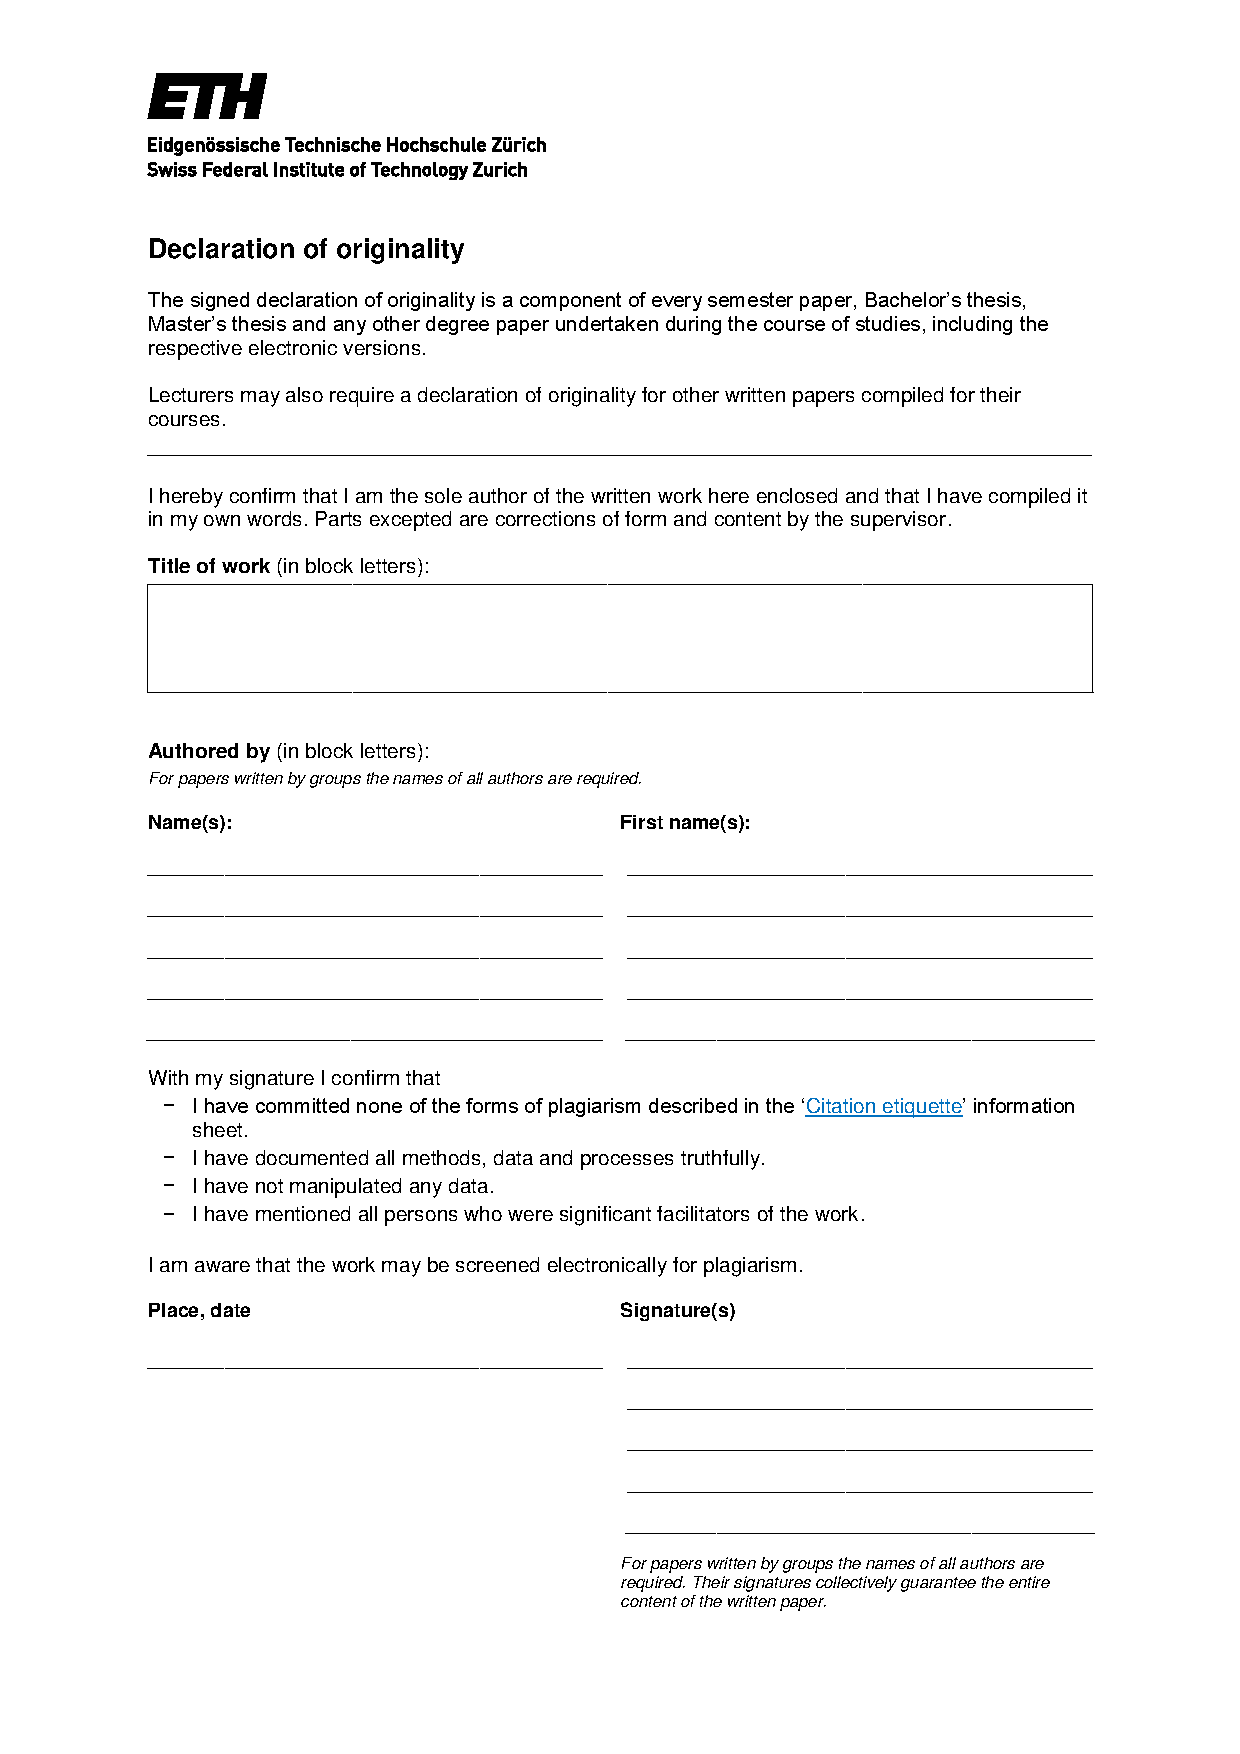
\includepdf[pages={-}]{declaration-originality.pdf}
\chapter*{Independence}

\vspace{2cm} 

I confirm that this master's thesis is my own work and I have documented all sources and material used.\\ \vspace{5em}

\begin{flushright}
	Z{\"u}rich, Switzerland, 28.08.2023
\end{flushright}
\newpage
\chapter*{Acknowledgment}

example
\newpage
\chapter*{Abstract}

example


\newpage
\tableofcontents
\clearpage
\chapter*{List of Abbreviations}

\begin{tabular}{rl}
	CNN & Convolutional Neural Network\\
	GNN & Graph Neural Network\\
\end{tabular}

\clearpage
\listoffigures
\clearpage
\listoftables
\newpage~
\restoregeometry

\pagenumbering{arabic}
\setcounter{page}{1}
\chapter{Introduction}

example

\section{Example}

example 


\subsection{Subexample}

example 


\newpage~
\let\cleardoublepage\clearpage
\chapter{Results} \label{chap:results}

example

\section{Example}

example 

\subsection{Subexample}

example 



\clearpage
\newpage~
\let\cleardoublepage\clearpage
\chapter{Discussion} \label{chap:discussion}

example

\section{Example}

example 


\subsection{Subexample}

example 


\newpage~
\let\cleardoublepage\clearpage
\chapter{Methods and Materials} \label{chap:methods}

example

\section{Example}

example 


\subsection{Subexample}

example 


\clearpage
\newpage~
\printbibliography[
heading=bibintoc,
title={References}
] %Prints bibliography
\newpage~
\chapter*{Supplement}
\markboth{Supplement}{Supplement}
\addcontentsline{toc}{chapter}{Supplement}
\beginsupplement

example



\end{document}


